\باب{وقت کے ساتھ بدلتے میدان اور میکس ویل کے مساوات}
گزشتہ بابوں میں وقت کے ساتھ تبدیل نہ ہونے والے میدان یعنی میدانوں پر غور کیا گیا۔یہاں سے آگے اس کتاب میں وقت کے ساتھ تبدیل ہوتے میدانوں پر غور کیا جائے گا۔

دو نئے اصول پر غور کیا جائے گا۔پہلا اصول مائکل فیراڈے نے تجرباتی طور پر ثابت کیا جس کے تحت وقت کے ساتھ بدلتا مقناطیسی میدان، برقی میدان کو جنم دیتا ہے۔دوسرا قانون  جیمس کلارک میکس ویل کے کاوشوں سے حاصل ہوا جس کے تحت وقت کے ساتھ بدلتا برقی میدان، مقناطیسی میدان کو جنم دیتا ہے۔ اس باب میں برقی و مقناطیسیات کے چار ایسے مساوات پیش کئے جائیں گے جو میکس ویل کے نام سے منسوب ہیں۔

\حصہ{فیراڈے کا قانون}
جناب مائکل فیراڈے نے تجرباتی طور پر ثابت کیا کہ وقت کے ساتھ بدلتا مقناطیسی میدان، برقی میدان پیدا کرتا ہے۔\اصطلاح{قانون فیراڈے}\فرہنگ{قانون!فیراڈے}\فرہنگ{فیراڈے!قانون}\حاشیہب{Faraday's law}\فرہنگ{Faraday's law} کو مندرجہ ذیل مساوات پیش کرتی ہے۔
\begin{align}\label{مساوات_میکس_ویل_فیراڈے_قانون}
\textrm{\RL{محرک برقی دباو}}=-\frac{\dif \Phi}{\dif t}
\end{align}
اس قانون کے تحت کسی بھی بند راہ سے گزرتی مقناطیس بہاو  میں تبدیلی اس راہ پر برقی دباو پیدا کرتی ہے۔ایسی برقی دباو روایتی طور پر \اصطلاح{محرک برقی دباو}\فرہنگ{محرک برقی دباو}\حاشیہب{electromotive force, emf}\فرہنگ{electromotive force}\فرہنگ{emf} پکاری جاتی ہے۔محرک برقی دباو\حاشیہد{محرک برقی دباو کی اصطلاح روایتی طور پر ہر قسم کے منبع برقی دباو کے لئے استعمال کی جاتی ہے۔} کی قیمت  وقت کے ساتھ بند راہ سے گزرتی مقناطیسی بہاو کے تبدیلی کے برابر ہوتی ہے۔محرک برقی دباو کی اکائی وولٹ \عددیء{\si{\volt}} ہے۔ضروری نہیں کہ بند راہ موصل مادے کی ہی ہو، یہ فرضی  بند لکیر بھی ہو سکتی ہے۔



محرک برقی دباو مکمل برقی دور میں برقی رو پیدا کرنے کی صلاحیت رکھتا ہے۔محرک برقی دباو سے پیدا برقی رو، بند راہ میں مقناطیسی بہاو پیدا کرے گی جس کی سمت، راہ میں پہلے سے موجود مقناطیسی بہاو کے سمت، کی الٹ ہوتی ہے۔مساوات \حوالہ{مساوات_میکس_ویل_فیراڈے_قانون} میں منفی کی علامت اسی اصول کو بیان کرتی ہے کہ بند راہ میں محرک برقی دباو سے پیدا برقی رو ایسا مقناطیسی بہاو پیدا کرتی ہے جو پہلے سے موجود مقناطیسی بہاو کے الٹ سمت رکھتی ہے۔اس اصول کو \اصطلاح{لینز}\فرہنگ{قانون!لینز}\حاشیہد{یہ قانون 1834 میں جناب لینز نے پیش کیا۔}\فرہنگ{لینز کا قانون}\حاشیہب{Lenz's law}\فرہنگ{Lenz's law} کا اصول کہا جاتا ہے۔

کسی بھی بند راہ سے گزرتی کل مقناطیسی  بہاو میں تبدیلی مندرجہ ذیل وجوہات کی بنا ممکن ہے۔
\begin{itemize}
\item
وقت کے ساتھ تبدیل ہوتی کثافت مقناطیسی بہاو جو ساکن بند راہ سے گزرتی ہو۔
\item
ساکن مقناطیسی میدان اور بند راہ کا آپس میں اضافی حرکت۔ 
\item
مندرجہ بالا دونوں وجوہات۔
\end{itemize}

اگر بند راہ \عددیء{N} چکر کے لچھے پر مشتمل ہو جہاں ہر چکر میں سے \عددیء{\Phi} مقناطیسی بہاو گزرتی ہو تب فیراڈے کے قانون کو
\begin{align}\label{مساوات_میکس_ویل_فیراڈے_قانون_ب}
\textrm{\RL{محرک برقی دباو}}=-N\frac{\dif \Phi}{\dif t}
\end{align}
لکھا جا سکتا ہے۔ 

\begin{figure}
\centering
\includegraphics{figMaxwellEMFandVoltageDrop}
\caption{محرک برقی دباو اور برقی دباو کی پہچان۔}
\label{شکل_میکس_ویل_محرک_برقی_دباو_پہچان}
\end{figure}

شکل \حوالہ{شکل_میکس_ویل_محرک_برقی_دباو_پہچان} میں محرک برقی دباو کو \عددیء{e} سے ظاہر کیا گیا ہے۔اگر محرک برقی دباو کو مزاحمت \عددیء{R} کے ساتھ منسلک کیا جائے تو برقی دور میں \عددیء{i} برقی رو گزرے گی۔مزاحمت پر برقی دباو کو \عددیء{v_R} سے ظاہر کیا گیا ہے۔مزاحمت کے نچلے سرے کو برقی زمین تصور کرتے ہوئے مزاحمت کے اوپر والے سرے پر برقی دباو \عددیء{v_R} ہے۔مزاحمت میں برقی رو کی سمت برقی دباو \عددیء{v_R} کے مثبت سرے سے اس کے منفی سرے کی جانب ہے۔اوہم کے قانون کے تحت \عددیء{v_R=i R} ہو گا۔ اب ذرہ اس دور میں منبع طاقت کی طرف نظر ڈالتے ہیں۔یہاں برقی رو کی سمت \عددیء{e} کے منفی سرے سے مثبت سرے کی جانب ہے۔برقی دباو اور محرک برقی دباو میں یہی بنیادی فرق ہے۔جہاں کہیں پر بھی برقی رو، مثبت سے منفی برقی رو کی جانب ہوتی ہے، محرک برقی دباو میں اس کے بالکل الٹ ہوتا ہے۔

برقی دباو کی تعریف \عددیء{v=-\int \kvec{E}\cdot \dif \kvec{L}} سے آپ بخوبی واقف ہیں۔مندرجہ بالا حقائق کو مد نظر رکھتے ہوئے محرک برقی دباو کی تعریف یوں لکھی جائے گی۔
\begin{align}\label{مساوات_میکس_ویل_محرک_برقی_دباو_تعریف}
\textrm{\RL{محرک برقی دباو}}=\oint \kvec{E} \cdot \dif \kvec{L}
\end{align}
محرک برقی دباو بند راہ پر بیان کی جاتی ہے۔صفحہ \حوالہصفحہ{مساوات_توانائی_بند_راستا} پر مساوات \حوالہ{مساوات_توانائی_بند_راستا} کے تحت ساکن برقی میدان میں کسی بھی بند دائرے پر \عددیء{\kvec{E}} کا لکیری تکمل صفر کے برابر ہوتا ہے۔مساوات \حوالہ{مساوات_میکس_ویل_محرک_برقی_دباو_تعریف} کہتا ہے کہ غیر ساکن مقناطیسی میدان میں ایسا نہیں ہوتا اور کسی بھی بند دائرے پر \عددیء{\kvec{E}} کا لکیری تکمل اس راہ پر پیدا محرک برقی دباو دیتا ہے۔

مساوات \حوالہ{مساوات_میکس_ویل_فیراڈے_قانون} اور مساوات \حوالہ{مساوات_میکس_ویل_محرک_برقی_دباو_تعریف} سے
\begin{align}\label{مساوات_میکس_ویل_محرک_دباو_اور_گھٹاو_تعلق}
\textrm{\RL{محرک برقی دباو}}=\oint \kvec{E} \cdot \dif \kvec{L}=-\frac{\dif}{\dif t} \int_S \kvec{B} \cdot \dif \kvec{S}
\end{align}
حاصل ہوتا ہے جہاں \عددیء{\Phi} کی جگہ کثافت مقناطیسی بہاو \عددیء{\kvec{B}} کا سطحی تکمل استعمال کیا گیا۔

اگر بند راہ کو دائیں ہاتھ میں یوں پکڑا جائے کہ انگلیاں راہ پر چلنی کی سمت میں ہوں تب انگوٹھا راہ سے گھیرے سمتی سطح کی سمت میں ہو گا۔مندرجہ بالا مساوات کہتا ہے کہ کسی بھی سمتی سطح سے گزرتی مقناطیسی بہاو اگر بڑھ رہی ہو تب محرک برقی دباو سطح کے سرحد پر مثبت سمت کے الٹ جانب برقی رو پیدا کرے گا۔مساوات \حوالہ{مساوات_میکس_ویل_محرک_دباو_اور_گھٹاو_تعلق} استعمال کرتے ہوئے دائیں ہاتھ کے اس قانون کو یاد رکھیں۔ 

آئیں وقت کے ساتھ تبدیل ہوتے مقناطیسی میدان کی وجہ سے پیدا ساکن بند راہ میں محرک برقی دباو پر پہلے غور کریں اور بعد میں ساکن مقناطیسی میدان میں حرکت کرتے راہ کی وجہ سے پیدا محرک برقی دباو پر غور کریں۔

ساکن راہ کی صورت میں مساوات \حوالہ{مساوات_میکس_ویل_محرک_دباو_اور_گھٹاو_تعلق} میں دائیں ہاتھ پر \عددیء{\kvec{B}} ہی وقت کے ساتھ تبدیل ہو رہی ہے یوں اس مساوات میں تفرق کے عمل کو تکمل کے اندر لے جایا جا سکتا ہے یعنی
 \begin{align}\label{مساوات_میکس_ویل_پہلی_مساوات_تکمل_صورت}
\textrm{\RL{محرک برقی دباو}}=\oint \kvec{E} \cdot \dif \kvec{L}=- \int_S \frac{\partial\kvec{B} }{\partial t}\cdot \dif \kvec{S}
\end{align}
آگے بڑھنے سے پہلے اس مساوات کی نقطہ شکل حاصل کرتے ہیں۔مساوات کے بائیں ہاتھ پر مسئلہ سٹوکس کے اطلاق سے
\begin{align*}
\int_S \left(\nabla \times \kvec{E} \right) \cdot \dif \kvec{S}=-\int_S \frac{\partial \kvec{B}}{\partial t} \cdot \dif \kvec{S}
\end{align*}
حاصل ہوتا ہے۔یاد رہے کہ سطح \عددیء{S} ایسی کوئی بھی سطح ہو سکتی ہے جس کا سرحد بند راہ ہو۔یوں ہم دونوں جانب مختلف سطحیں لے سکتے ہیں جب تک دونوں سطحوں کے سرحد یہی بند راہ ہو۔اسی طرح ہم ایک ہی سطح کو دونوں جانب تکمل میں استعمال کر سکتے ہیں۔یہ مساوات کسی بھی سطح کے لئے درست ہے لہٰذا یہ تفرقی سطح \عددیء{\dif \kvec{S}} کے لئے بھی درست ہے۔تفرقی سطح کے لئے اسے یوں
\begin{align*}
\left(\nabla \times \kvec{E} \right) \cdot \dif \kvec{S}=-\frac{\partial \kvec{B}}{\partial t} \cdot \dif \kvec{S}
\end{align*}
یعنی
\begin{align}\label{مساوات_میکس_ویل_پہلی_مساوات_نقطہ_صورت}
\nabla \times \kvec{E}=-\frac{\partial \kvec{B}}{\partial t}
\end{align}
لکھا جا سکتا ہے۔

مساوات \حوالہ{مساوات_میکس_ویل_پہلی_مساوات_نقطہ_صورت} میکس ویل کے چار مساواتوں میں سے  پہلی مساوات\فرہنگ{میکس ویل!پہلی مساوات}\فرہنگ{Maxwell!first equation} ہے۔یہ میکس ویل کے پہلی مساوات کی نقطہ شکل ہے۔اس مساوات کی نقطہ شکل ہی عموماً استعمال ہوتی ہے۔میکس ویل کے پہلی مساوات کی  تکمل شکل مساوات \حوالہ{مساوات_میکس_ویل_پہلی_مساوات_تکمل_صورت} بیان کرتی ہے۔وقت کے ساتھ نہ تبدیل ہوتے مقناطیسی میدان کی صورت میں مساوات \حوالہ{مساوات_میکس_ویل_پہلی_مساوات_نقطہ_صورت} اور مساوات \حوالہ{مساوات_میکس_ویل_پہلی_مساوات_تکمل_صورت} ساکن میدان کے مساوات کی صورت اختیار کرتے ہیں یعنی
\begin{align}
\oint \kvec{E} \cdot \dif \kvec{L}=0 \quad \quad (\textrm{\RL{برقی سکون}})
\end{align}
اور
\begin{align*}
\nabla \times \kvec{E}=0 \quad \quad (\textrm{\RL{برقی سکون}})
\end{align*}
%=======================

آئیں مساوات \حوالہ{مساوات_میکس_ویل_پہلی_مساوات_تکمل_صورت} اور مساوات \حوالہ{مساوات_میکس_ویل_پہلی_مساوات_نقطہ_صورت} کو استعمال کر کے دیکھیں۔تصور کریں کہ  \عددیء{\rho<\rho_2} نلکی خطے میں وقت کے ساتھ مسلسل بڑھتی
\begin{align}\label{مساوات_میکس_ویل_غیر_حقیقی_میدان}
\kvec{B}=B_0 e^{kt} \az \quad \quad (\rho < \rho_2)
\end{align}
کثافت مقناطیسی بہاو پائی جاتی ہے  جہاں \عددیء{B_0} ایک مستقل ہے۔ ہم \عددیء{z=0} سطح پر \عددیء{\rho_1} رداس کی گول راہ لیتے ہیں۔مشابہت سے ہم کہہ سکتے ہیں کہ اس پورے راہ پر \عددیء{E_\phi} کی قیمت تبدیل نہیں ہو سکتی لہٰذا مساوات \حوالہ{مساوات_میکس_ویل_پہلی_مساوات_تکمل_صورت}  سے 
\begin{align*}
\textrm{\RL{محرک برقی دباو}}=2\pi \rho_1 E_{\phi}=-k B_0 e^{k t} \pi \rho_1^2
\end{align*}
حاصل ہوتا ہے۔یوں کسی بھی رداس پر برقی میدان کی شدت
\begin{align}
\kvec{E}=-\frac{1}{2} k B_0 e^{kt} \rho \aphi
\end{align}
لکھی جا سکتی ہے۔

آئیں اب یہی جواب مساوات \حوالہ{مساوات_میکس_ویل_پہلی_مساوات_نقطہ_صورت} سے حاصل کریں۔چونکہ اس مساوات کے دائیں جانب صرف \عددیء{\az} جزو پایا جاتا ہے لہٰذا بائیں ہاتھ بھی صرف یہی جزو ہو گا لہٰذا اس مساوات سے
\begin{align*}
\frac{1}{\rho} \frac{\partial (\rho E_{\phi})}{\partial \rho}=-k B_0 e^{kt}
\end{align*}
لکھا جا سکتا ہے۔دونوں اطراف کو \عددیء{\rho} سے ضرب دیتے ہوئے  \عددیء{0} تا \عددیء{\rho} تکمل لے کر
\begin{align*}
\rho E_{\phi}=-k B_0 e^{k t} \frac{\rho^2}{2}
\end{align*}
یعنی
\begin{align}
\kvec{E}=-\frac{1}{2} k B_0 e^{kt} \rho \aphi
\end{align}
ہی دوبارہ حاصل ہوتا ہے جہاں رداسی تکمل میں \عددیء{t} مستقل کا کردار ادا کرتا ہے۔

مثبت \عددیء{B_0} کی صورت میں اس راہ پر \عددیء{\aphi} کی الٹ سمت میں برقی رو گزرے گی جو \عددیء{\az} کی الٹ سمت میں کثافت مقناطیسی بہاو پیدا کرتے ہوئے پہلے سے موجود مقناطیسی میدان میں تبدیلی کو روکنے کی کوشش کرتی ہے۔

اس مثال کے آخر میں یہ بتلانا ضروری ہے کہ مساوات \حوالہ{مساوات_میکس_ویل_غیر_حقیقی_میدان} میں دیا گیا میدان غیر حقیقی ہے چونکہ یہ میکس ویل کے دیگر مساوات پر پورا نہیں اترتا۔

\begin{figure}
\centering
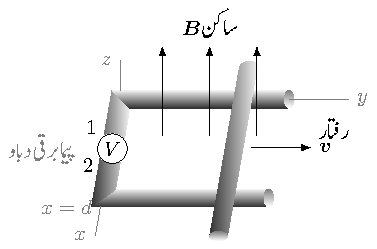
\includegraphics{figMaxwellSlidingConductorInStaticField}
\caption{وقت کے ساتھ نہ تبدیل ہوتے یکساں مقناطیسی میدان میں حرکت کرتے موصل سلاخ پر محرک برقی دباو پیدا ہوتی ہے۔}
\label{شکل_میکس_ویل_محرک_سلاخ_محرک_دباو}
\end{figure}

آئیں اب ایسی مثال دیکھیں جس میں وقت کے ساتھ تبدیل نہ ہونے والے مقناطیسی میدان میں  بند راہ حرکت کر رہی ہو۔شکل \حوالہ{شکل_میکس_ویل_محرک_سلاخ_محرک_دباو} میں ایسی صورت حال دکھائی گئی ہے۔اس شکل میں \عددیء{\kvec{v}} سمتی رفتار کو جبکہ \عددیء{V} برقی دباو ناپنے کی آلہ\حاشیہد{وولٹ میٹر} یعنی \اصطلاح{پیما برقی دباو}\فرہنگ{پیما!برقی دباو}\فرہنگ{برقی دباو!پیما}\حاشیہب{voltmeter}\فرہنگ{voltmeter} کو ظاہر کرتی ہے۔اس شکل میں دو افقی اور دو متوازی موصل سلاخ بند راہ یا بند دور بناتے ہیں۔ متوازی افقی سلاخوں کو بائیں طرف عمودی سلاخ سے جوڑا گیا ہے جس میں قابل نظر انداز جسامت اور لامحدود مزاحمت والا پیما برقی دباو نسب ہے، جبکہ دائیں جانب انہیں \عددیء{\kvec{v}} سمتی رفتار سے حرکت کرتے عمودی سلاخ سے جوڑا گیا ہے۔وقت کے ساتھ نہ تبدیل ہوتا اور ہر جگہ یکساں کثافت مقناطیسی بہاو \عددیء{\kvec{B}} بند راہ کی گھیرے سطح کے عمودی ہے۔

مثبت \عددیء{\kvec{B}} کی صورت میں \عددیء{\kvec{B}} کی سمت ہی بند راہ سے گھیری گئی سطح کی سمت ہو گی اور بند راہ کی سمت گھڑی کے الٹ ہو گی۔یوں راہ کے مثبت سمت میں دائیں ہاتھ کی انگلیاں رکھتے ہوئے گھیری سطح کی سمت انگوٹھے سے حاصل کی جاتی ہے۔ 

کسی بھی لمحہ \عددیء{t} پر حرکت کرتے سلاخ کے مقام کو \عددیء{y} سے ظاہر کرتے ہوئے ہم \عددیء{y=v t} لکھ سکتے ہیں جہاں \عددیء{v} سلاخ کے رفتار کی قیمت ہے۔یوں لمحہ \عددیء{t} پر بند دور کا ارتباط بہاو
\begin{align*}
\Phi=B d y =B d v t
\end{align*} 
ہو گا جو مساوات \حوالہ{مساوات_میکس_ویل_فیراڈے_قانون} کے تحت بند دور میں
\begin{align*}
e=-\frac{\dif \Phi}{\dif t}=-B d v
\end{align*}
محرک برقی دباو \عددیء{e} پیدا کرے گا۔

اب محرک برقی دباو \عددیء{\oint \kvec{E}\cdot \dif \kvec{L}} کو کہتے ہیں لہٰذا مندرجہ بالا جواب راہ پر گھڑی کے الٹ سمت میں اس بند لکیری تکمل سے بھی حاصل ہونا چاہیے۔ہم دیکھ چکے ہیں کہ برقی سکون کی صورت میں موصل کی سطح پر سطح کے متوازی \عددیء{E} صفر رہتی ہے۔ہم آگے دیکھیں گے کہ وقت کے ساتھ تبدیل ہوتے برقی میدان میں بھی موصل کی سطح پر متوازی \عددیء{E} صفر ہی رہتی ہے۔یوں شکل \حوالہ{شکل_میکس_ویل_محرک_سلاخ_محرک_دباو} پر گھڑی کے الٹ چلتے ہوئے تمام سلاخوں پر تکمل کی قیمت صفر کے برابر ہو گی۔پیما برقی دباو کی مزاحمت صفر نہیں ہے لہٰذا تکمل کی قیمت پیما برقی دباو پر مندرجہ بالا قیمت کے برابر ہونا ہو گا۔گھڑی کی الٹ سمت چلتے ہوئے پیما برقی دباو کی لمبائی کو \عددیء{\dif \kvec{L}} لکھتے ہوئے ہم دیکھتے ہیں کہ \عددیء{\kvec{E} \cdot \dif \kvec{L}=-B d v} ہونا ہو گا۔چونکہ \عددیء{\dif \kvec{L}=\dif L \ax} کے برابر ہے لہٰذا \عددیء{\kvec{E}} کی سمت \عددیء{\ax} کے الٹ ہو گی۔یوں پیما برقی دباو پر \عددیء{\kvec{E}} کی سمت پیما کے دوسرے سرے سے پہلے سرے کی جانب ہے اور پیما پر برقی دباو کا مثبت سرا پیما کا دوسرا سرا ہے۔

پیما کی جگہ مزاحمت جوڑنے سے دور میں گھڑی کے الٹ برقی رو گزرے گی جو \عددیء{\az} کے الٹ سمت میں مقناطیسی بہاو پیدا کرے گی۔یہ لورنز کے قانون کے عین مطابق ہے۔

آئیں اب اسی شکل میں دئے مسئلے کو حرکی برقی دباو تصور کرتے ہوئے حل کریں۔مقناطیسی میدان میں \عددیء{\kvec{v}} سمتی رفتار سے حرکت کرتے ہوئے چارج \عددیء{Q} پر قوت
\begin{align*}
\kvec{F}=Q \kvec{v} \times \kvec{B}
\end{align*}
یا حرکی شدت \عددیء{\kvec{E}_{\textrm{حرکی}}}
\begin{align}
\kvec{E}_{\textrm{حرکی}}=\frac{\kvec{F}}{Q}=\kvec{v} \times \kvec{B}
\end{align}
عمل کرتی ہے۔حرکی شدت \عددیء{\ax} سمت میں ہے۔حرکت کرتے سلاخ میں ساکن مثبت ایٹم اور آزاد منفی الیکٹران پائے جاتے ہیں۔ان تمام چارجوں  پر ایسی قوت پائی جائے گی البتہ ساکن ایٹم مقید ہونے کی بنا حرکت نہیں کریں گے۔اگر محرک سلاخ کو متوازی سلاخوں سے اٹھایا جائے تو اس میں آزاد الیکٹران پر \عددیء{\ax} کے الٹ جانب قوت انہیں سلاخ کے پرلے سرے پر انبار کرنا شروع کر دے گی۔الیکٹرانوں کا انبار سلاخ میں \عددیء{-\ax} جانب برقی میدان کی شدت \عددیء{\kvec{E}_{\textrm{ساکن}}} پیدا کرے گا۔الیکٹران کا انبار بڑھتا رہے گا حتیٰ کہ  \عددیء{\kvec{E}_{\textrm{حرکی}}} اور \عددیء{\kvec{E}_{\textrm{ساکن}}} برابر ہو جائیں۔ایسا ہوتے ہی سلاخ میں کل برقی میدان کی شدت صفر ہو جائے گی اور اس میں چارج کا حرکت رک جائے گا۔

یوں حرکی برقی دباو
\begin{align}
\textrm{\RL{محرک برقی دباو}}=\oint \kvec{E}_{\textrm{حرکی}} \cdot \dif \kvec{L}=\oint \left(\kvec{v} \times \kvec{B} \right) \cdot \dif \kvec{L}
\end{align} 
سے حاصل ہو گی۔مساوات کے دائیں ہاتھ بند راہ کے ساکن حصوں پر تکمل کی قیمت صفر ہو گی لہٰذا محرک برقی دباو صرف حرکت کرتے حصوں کی وجہ سے پیدا ہو گی۔یوں حرکت کرتے سلاخ پر گھڑی کے الٹ چلتے ہوئے تکمل سے
\begin{align*}
\oint \left(\kvec{v} \times \kvec{B} \right) \cdot \dif \kvec{L}=\int_d^0 v B \dif x=-B v d
\end{align*}
حاصل ہوتا ہے ۔چونکہ \عددیء{\kvec{B}} اذ خود وقت کے ساتھ تبدیل نہیں ہو رہا لہٰذا یہی کل محرک برقی دباو ہو گا۔

یوں وقت کے ساتھ تبدیل نہ ہوتے مقناطیسی میدان میں حرکت کرتے بند راہ میں محرک برقی دباو حاصل کرتے وقت حرکت کرتے حصوں پر حرکی شدت \عددیء{\kvec{E}_{\textrm{حرکی}}} کے استعمال سے محرک برقی دباو یوں
\begin{align}
\textrm{\RL{محرک برقی دباو}}=\oint \kvec{E} \cdot \dif \kvec{L}=\oint \kvec{E}_{\textrm{حرکی}} \cdot \dif \kvec{L}=\oint \left(\kvec{v} \times \kvec{B} \right) \cdot \dif \kvec{L}
\end{align} 
حاصل کی جا سکتی ہے۔البتہ وقت کے ساتھ بدلتی مقناطیسی میدان میں محرک برقی دباو کے حصول میں مساوات \حوالہ{مساوات_میکس_ویل_پہلی_مساوات_تکمل_صورت} کا حصہ شامل کرنا ضروری ہے یوں محرک برقی دباو
\begin{align}
\textrm{\RL{محرک برقی دباو}}=\oint \kvec{E} \cdot \dif \kvec{L}=-\int_S \frac{\partial \kvec{B}}{\partial t} \cdot \dif \kvec{S}+\oint \left(\kvec{v} \times \kvec{B} \right) \cdot \dif \kvec{L}
\end{align} 
سے حاصل ہو گی۔یہ مساوات دراصل مساوات \حوالہ{مساوات_میکس_ویل_فیراڈے_قانون}
\begin{align*}
\textrm{\RL{محرک برقی دباو}}=-\frac{\dif \Phi}{\dif t}
\end{align*}
ہی ہے۔

اگرچہ مساوات \حوالہ{مساوات_میکس_ویل_فیراڈے_قانون} انتہائی سادہ شکل رکھتی ہے لیکن اس کا استعمال کبھی کبھار مشکل ہو جاتا ہے۔ایسا اس وقت ہوتا ہے جب دور کے کسی حصے کو تبدیل کرتے ہوئے دوسرا حصہ نسب کیا جائے۔یہ بات شکل \حوالہ{شکل-میکس_ویل_سوئچ_سے_محرک_دباو_نہیں_پیدا_ہوتی} پر غور کرنے سے بہتر سمجھ آئے گی۔اس شکل میں نا تو وقت کے ساتھ تبدیل ہوتا مقناطیسی میدان ہے اور نا ہی بند راہ کا کوئی حصہ متحرک ہے۔البتہ شکل میں دکھائے سوئچ کو چالو یا غیر چالو کرتے ہوئے بند راہ میں مقناطیسی بہاو کم اور زیادہ کیا جا سکتا ہے۔یہاں بغیر سوچے مساوات \حوالہ{مساوات_میکس_ویل_فیراڈے_قانون} استعمال کرتے ہوئے غلط نتائج حاصل ہوتے ہیں۔ یاد رہے کہ برقی دباو یا تو وقت کے ساتھ بدلتے مقناطیسی میدان اور یا پھر بند راہ کے کسی حصے کے حرکت سے ہی پیدا ہو گا۔
  
\begin{figure}
\centering
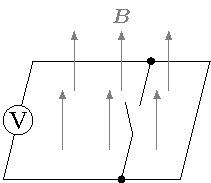
\includegraphics{figMaxwellSwitchingCoductorsToChangeFlux}
\caption{محرک برقی دباو یا تا وقت کے ساتھ بدلتی مقناطیسی میدان اور یا حرکت کرتے بند راہ سے ہی پیدا ہو سکتی ہے۔}
\label{شکل-میکس_ویل_سوئچ_سے_محرک_دباو_نہیں_پیدا_ہوتی}
\end{figure}

%==============
\ابتدا{مشق}
شکل \حوالہ{شکل-میکس_ویل_سوئچ_سے_محرک_دباو_نہیں_پیدا_ہوتی} میں \عددیء{\kvec{B}=0.5\az } ٹسلا، رفتار \عددیء{100 y \ay} میٹر فی سیکنڈ جبکہ \عددیء{d=0.5} میٹر ہے۔اگر \عددیء{t=0} پر \عددیء{y=0.2} میٹر ہو تب \عددیء{t=15} ملی سیکنڈ پر مندرجہ ذیل حاصل کریں۔
\begin{itemize}
\item
سلاخ کی رفتار،
\item
محرک برقی دباو \عددیء{V_{21}}،
\item
پیما برقی دباو کی اندرونی مزاحمت دس میگا اوہم کی صورت میں دور میں برقی رو۔
\end{itemize} 

جوابات:\عددیء{\SI{4.017}{\meter\per\second}}، \عددیء{\SI{100}{\volt}}، \عددیء{\SI{10}{\micro \ampere}}

\انتہا{مشق}
%=======================

\حصہ{انتقالی برقی رو}
فیراڈے کے تجرباتی نتیجے سے میکس ویل کی پہلی مساوات
\begin{align}
\nabla \times \kvec{E}=-\frac{\partial \kvec{B}}{\partial t}
\end{align}
حاصل ہوئی جو کہتا ہے کہ بدلتی مقناطیسی میدان پیدا کرتا ہے برقی دباو۔گردش کے عمل کو مد نظر رکھتے ہوئے ہم دیکھتے ہیں ایسے پیدا کردہ برقی دباو کا بند لکیری تکمل صفر کے برابر نہیں ہوتا۔ آئیں اب وقت کے ساتھ تبدیل ہوتے برقی میدان پر غور کریں۔

ایمپیئر کے دوری قانون کی نقطہ شکل
\begin{align}\label{مساوات_میکس_ویل_ایمپیئر_دوری_نقطہ_صورت}
\nabla \times \kvec{H}=\kvec{J}
\end{align}
ساکن مقناطیسی میدان پر لاگو ہوتی ہے۔اس مساوات کی پھیلاو
\begin{align*}
\nabla \cdot \nabla \times \kvec{H}=0=\nabla \cdot \kvec{J}
\end{align*}
 لیتے ہوئے ہم دیکھتے ہیں کہ گردش کی پھیلاو ہر صورت صفر کے برابر ہوتی ہے لہٰذا مندرجہ بالا مساوات کا بایاں ہاتھ ہر صورت صفر دے گا اور یوں اگر یہ مساوات درست ہو تب اس کا دایاں ہاتھ بھی ہر صورت صفر ہونا چاہیے۔مگر ہم استمراری  مساوات سے جانتے ہیں کہ
\begin{align}
\nabla \cdot \kvec{J}=-\frac{\partial \rho}{\partial t}
\end{align} 
ہوتا ہے۔اس سے ثابت ہوتا ہے کہ مساوات \حوالہ{مساوات_میکس_ویل_ایمپیئر_دوری_نقطہ_صورت} صرف اس صورت درست ہو گا جب \عددیء{\tfrac{\partial \rho}{\partial t}=0} ہو۔یہ ایک غیر ضروری اور غیر حقیقی شرط ہے لہٰذا وقت کے ساتھ تبدیل ہوتے برقی میدان پر استعمال کے قابل بنانے کی خاطر  مساوات \حوالہ{مساوات_میکس_ویل_ایمپیئر_دوری_نقطہ_صورت} کو تبدیل کرنا لازم ہے۔تصور کریں کہ مساوات \حوالہ{مساوات_میکس_ویل_ایمپیئر_دوری_نقطہ_صورت} میں نا معلوم جزو \عددیء{\kvec{G}} کی شمولیت سے یہ مساوات وقت  کے ساتھ تبدیل ہوتے برقی میدان پر بھی لاگو کرنے کے قابل ہو جاتا ہے۔ایسی صورت میں مساوات \حوالہ{مساوات_میکس_ویل_ایمپیئر_دوری_نقطہ_صورت} یوں
\begin{align*}
\nabla \times \kvec{H}=\kvec{J}+\kvec{G}
\end{align*}
لکھی جائے گی۔آئیں دوبارہ اس کی پھیلاو حاصل کریں جس سے
\begin{align*}
0=\nabla \cdot \kvec{J}+\nabla \cdot \kvec{G}
\end{align*}
یا
\begin{align*}
\nabla \cdot \kvec{G}=\frac{\partial \rho}{\partial t}
\end{align*}
حاصل ہوتا ہے جہاں استمراری مساوات کا سہارا لیا گیا۔اس مساوات میں \عددیء{\rho} کی جگہ \عددیء{\nabla \cdot \kvec{D}} پر کرنے سے
\begin{align*}
\nabla \cdot \kvec{G}=\frac{\partial \left(\nabla \cdot \kvec{D} \right)}{\partial t}=\nabla \cdot \frac{\partial \kvec{D}}{\partial t}
\end{align*}
یعنی
 \begin{align*}
\kvec{G}=\frac{\partial \kvec{D}}{\partial t}
\end{align*}
حاصل ہوتا ہے۔یوں ایمپیئر کے دوری قانون کی درست شکل
\begin{align}\label{مساوات-میکس_ویل_دوسری_مساوات_نقطہ_شکل}
\nabla \times \kvec{H}=\kvec{J}+\frac{\partial \kvec{D}}{\partial t}
\end{align}
ہے۔ مندرجہ بالا مساوات برقی و مقناطیسیات کے اب تک تمام دریافت کردہ اصولوں پر پورا اترتی آئی ہے۔

مساوات \حوالہ{مساوات-میکس_ویل_دوسری_مساوات_نقطہ_شکل} میکس ویل کے مساوات میں سے ایک مساوات ہے۔اس مساوات میں \عددیء{\tfrac{\partial \kvec{D}}{\partial t}} کی بُعد ایمپیئر فی مربع میٹر حاصل ہوتی ہے جو کثافت برقی رو کا بُعد ہے۔میکس ویل نے اس مساوات میں دائیں ہاتھ نئے جزو  کو \اصطلاح{انتقالی رو}\فرہنگ{انتقالی رو}\حاشیہب{displacement current}\فرہنگ{displacement current} کا نام دیا اور \عددیء{\kvec{J}_d} سے ظاہر کیا یعنی
\begin{align*}
\nabla \times \kvec{H}&=\kvec{J}+\kvec{J}_d\\
\kvec{J}_d&=\frac{\partial \kvec{D}}{\partial t}
\end{align*}
